% arara: pdflatex: { synctex: yes }
% arara: makeindex: { style: ctuthesis }
% arara: bibtex

% The class takes all the key=value arguments that \ctusetup does,
% and a couple more: draft and oneside
\documentclass[twoside]{ctuthesis}
\usepackage{graphicx}
\usepackage{listings}
\usepackage{mathtools}
\raggedbottom % This prevents text from sticking to the bottom of pages! Finally!


\ctusetup{
%	preprint = \ctuverlog,
	mainlanguage = english,
%	titlelanguage = czech,
%	mainlanguage = czech,
	otherlanguages = {czech},
	title-czech = {},
	title-english = {Alcohol content measurement within the fermentation process},
	subtitle-czech = {},
	subtitle-english = {\textit{Low-cost automatic ethanol measurement as indication of fermentation progress}},
	doctype = B,
	faculty = F3,
	department-czech = {Department in Czech},
	department-english = {Department of Control Engineering},
	author = {Gil Goldman},
	supervisor = {Prof. Jiři Novák},
	supervisor-address = {Technicka 2\\ 166 27\\ Praha 6},
	fieldofstudy-english = {Robotics and Cybernetics},
	subfieldofstudy-english = {Control Engineering},
	fieldofstudy-czech = {Robotika a Kybernetika},
	subfieldofstudy-czech = {},
	keywords-czech = {Fermentace, Ethanol, Automatizace, Měření},
	keywords-english = {Fermentation, Ethanol, Automation, Measurement},
	day = 20,
	month = 4,
	year = 2018,
	specification-file = {ctutest-zadani.pdf},
%	front-specification = true,
%	front-list-of-figures = false,
%	front-list-of-tables = false,
%	monochrome = true,
%	layout-short = true,
}

\ctuprocess

\addto\ctucaptionsczech{%
	\def\supervisorname{Vedoucí}%
	\def\subfieldofstudyname{Studijní program}%
}

\ctutemplateset{maketitle twocolumn default}{
	\begin{twocolumnfrontmatterpage}
		\ctutemplate{twocolumn.thanks}
		\ctutemplate{twocolumn.declaration}
		\ctutemplate{twocolumn.abstract.in.titlelanguage}
		\ctutemplate{twocolumn.abstract.in.secondlanguage}
		\ctutemplate{twocolumn.tableofcontents}
		\ctutemplate{twocolumn.listoffigures}
	\end{twocolumnfrontmatterpage}
}

% Theorem declarations, this is the reasonable default, anybody can do what they wish.
% If you prefer theorems in italics rather than slanted, use \theoremstyle{plainit}

\theoremstyle{plain}
\newtheorem{theorem}{Theorem}[chapter]
\newtheorem{corollary}[theorem]{Corollary}
\newtheorem{lemma}[theorem]{Lemma}
\newtheorem{proposition}[theorem]{Proposition}

\theoremstyle{definition}
\newtheorem{definition}[theorem]{Definition}
\newtheorem{example}[theorem]{Example}
\newtheorem{conjecture}[theorem]{Conjecture}

\theoremstyle{note}
\newtheorem*{remark*}{Remark}
\newtheorem{remark}[theorem]{Remark}

%\setlength{\parskip}{5ex plus 0.2ex minus 0.2ex}

% Abstract in Czech
\begin{abstract-czech}
V této práci budu prozkoumávat moderní metody měření postupu fermentačních procesů v mikropivovaru. Dále budu implementovat  a testovat automatické řešení na monitorování postupné akumulace ethanolu během procesu fermentace piva.
\end{abstract-czech}

% Abstract in English
\begin{abstract-english}
 This dissertation surveys the current methods of measuring the progression of micro-brewed beer fermentation processes. In addition, it describes the automatic solution I implemented to monitor the gradual accumulation of ethanol in the process of beer fermentation.
\end{abstract-english}

% Acknowledgements / Podekovani
\begin{thanks}
The Author would like to thank Doc. Ing. Jiri Novak, Ph.D. for his thorough guidance and tutelage - it has been an honor working on this topic under his supervision. In addition, the author would like to thank Doc. Ing. Mattia Butta, Ph.D. for his patient and kind assistance with the measurements, and Richard Sedivy, Esq. for his translation of relevant parts into Czech. Furthermore, the author would like to note the assistance of Ido Schwartz and Ohad Barta with the experimental parts, and Eran Goldman-Malka with technical matters.%\emph{alma mater}.
\end{thanks}

% Declaration / Prohlaseni
\begin{declaration}

Prohlašuji, že jsem předloženou práci vypracoval samostatně, a že jsem uvedl veškerou použitou literaturu.\\
V Praze, \ctufield{day}.~\monthinlanguage{title}~\ctufield{year}\\

\vspace{5mm} % a small space between both paragraphs

I declare that this work is all my own work and I have cited all the sources I have
used in the bibliography.\\

In Prague, \ctufield{day}.~\monthinlanguage{title}~\ctufield{year}

\end{declaration}

% Only for testing purposes
\listfiles
\usepackage[pagewise]{lineno}
\usepackage{lipsum,blindtext}
\usepackage{mathrsfs} % provides \mathscr used in the ridiculous examples

\begin{document}

\maketitle

\section{Introduction}

In this dissertation I will provide a brief overview of the way beer is made by home brewers today - I will follow the process from grains to beer and observe a few issues with the common way this process is carried out today in most microbreweries.\\
Then, I will explore the various ways by which ethanol is currently being measured in home-grade brewing processes, also known as micro-brewing, and evaluate the advantages and disadvantages of each method. I will then discuss why and how the method suggested by this paper is the most suitable.\\
I will then establish and justify an automatic, low cost solution to the issue of accurate and safe ethanol measurement, followed by rigorous testing of the proposed solution.

\pagebreak

\begingroup
\renewcommand{\cleardoublepage}{}
\renewcommand{\clearpage}{}
\chapter{How beer is brewed}
\endgroup

In this chapter, I will elaborate on how beer is being made, and discuss the most common method of micro-brewing. From this explanation the core weakness in the process, and the justification for this thesis, is easily identifiable.

\section{Overview of Beer Brewing}
In general, micro-brewing can be seen as a fairly simple process, composed of five significant stages: \textit{Malting}, \textit{Mashing}, \textit{Worting}, \textit{Fermentation}, and \textit{Packing}.\\
A short flow chart below illustrates the brewing process:

\begin{figure}[H]
\centering
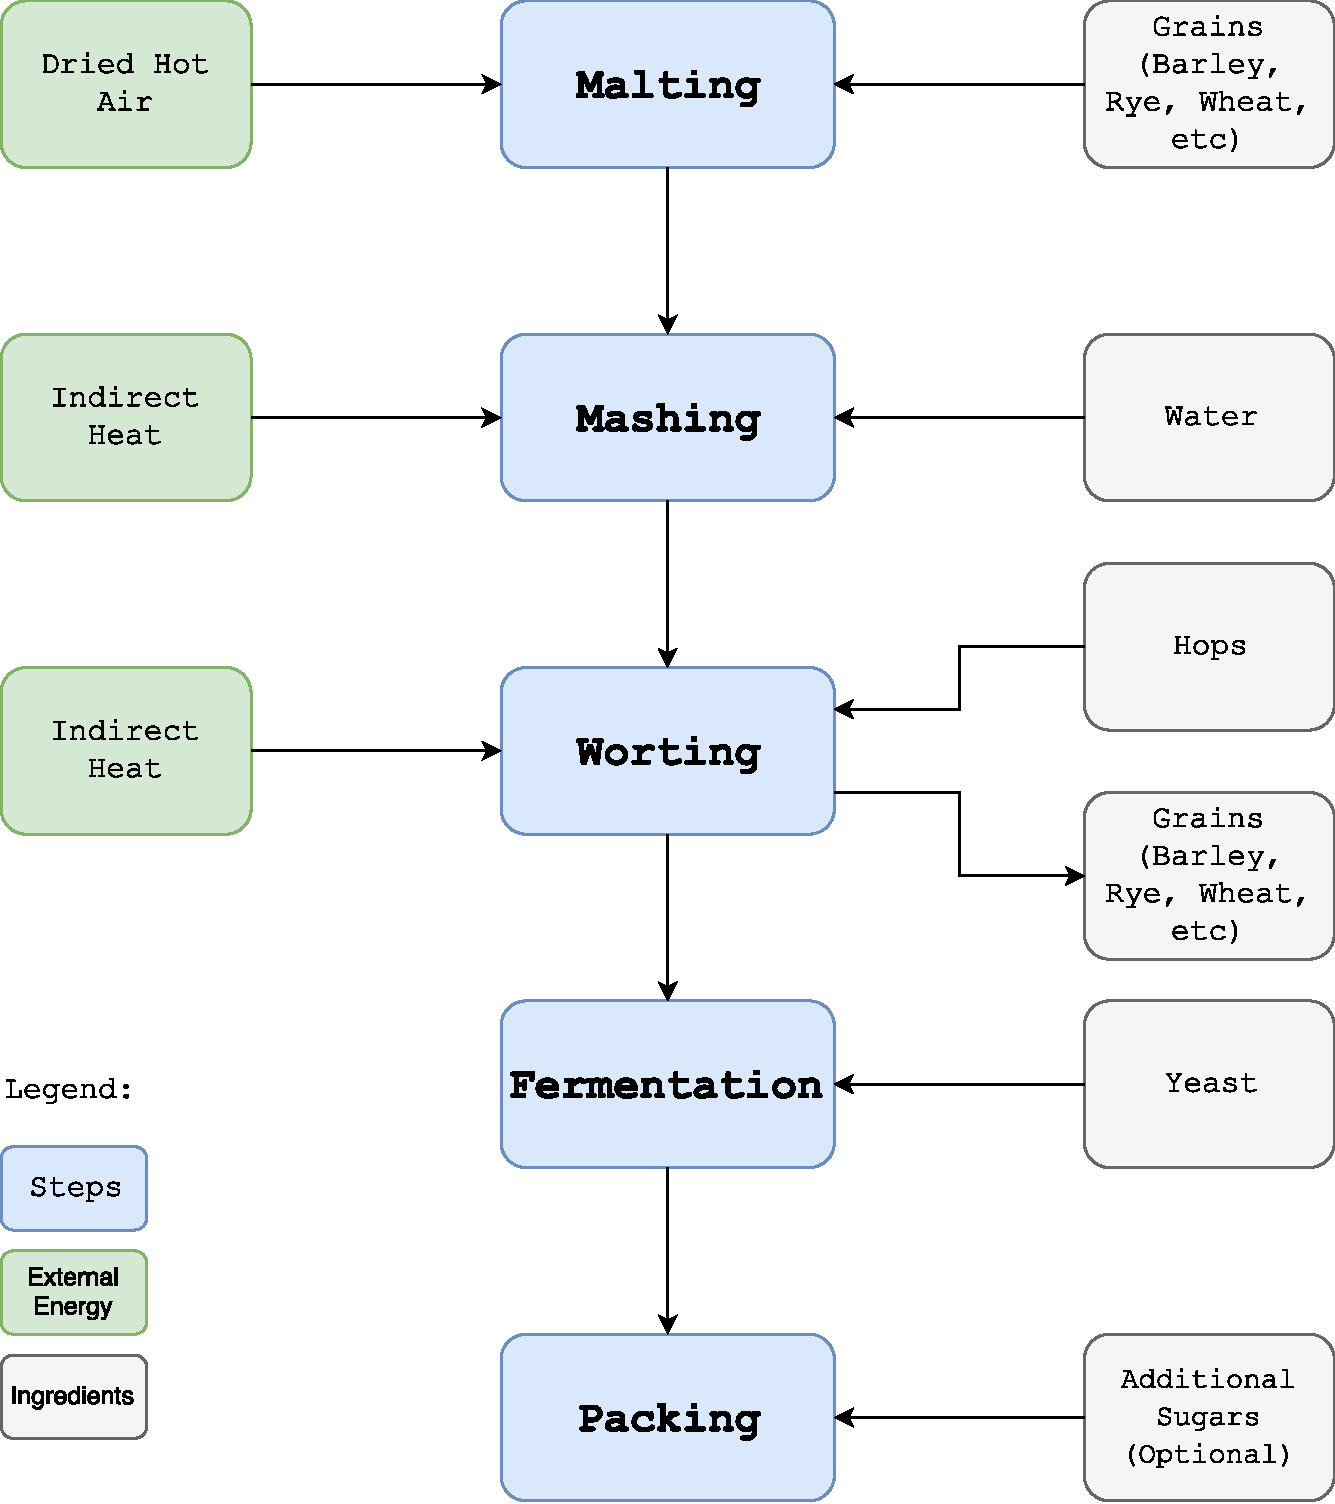
\includegraphics[scale = 0.39]{BeerMakingFlowChart}
\caption{Flow chart of the Brewing process}
\end{figure}


\section{Malting}
The first step in beer brewing is called \textit{Malting}, and it is the name given to the process of preparing the grain to be \textit{mashed}. The most common grains to be malted are Barley (\textit{Hordeum Vulgare}) and Wheat (\textit{Triticum aestivum}). Sorghum (\textit{Sorghum Vulgare}) is also rather common, but mostly in its indigenous continent of Africa. Some varieties of rye, oats, and millets are also used, but to a significantly lesser extent \cite{Brewing_Science}.\\
The main goal of malting is to germinate the grains used in the brewing process, breaking the $\alpha-amylase$ and $\beta-amylase$ enzymes out of the \textit{amylose homologous} series in the grains. These Enzymes will later be used to break the grain starches into various saccharides .\\
Malting is most commonly done by steeping the grains in and out of water until they reach about 45$\%$ moisture content, and then maintaining that high moisture content via bursts of highly humidified air. The germination process is stopped by $Kilning$ - blowing hot, dry air through the grains to reduce their inherent moisture content down to 5$\%$ \cite{Malting_Brewing}. Various flavors and colors can be developed by changing the duration and temperature of the Kilning process. \cite{Malting} \\
The final step of the Malting process is done as close to brewing as feasible, and involves cracking and grinding the grains to allow easy extraction of the starches during the Mashing stage. The end product of this process is called $Malt$.\\
As this process is relatively expensive and mechanically demanding, the majority of micro-breweries buy malt rather than produce it.

\section{Mashing}
The process of $mashing$ involves steeping, or cooking, the malt in water at specific temperatures to allow the enzymes developed during the malting process to take effect.\\
The $\alpha-amylase$ enzyme's main function is to break the large, complex, insoluble starches in the grain into smaller, simpler, and soluble starches. The $\beta-amylase$ converts the water soluble starches into usable types of sugar, such as the monosaccharide glucose, the disaccharide maltose, the trisaccharide maltotriose, and various other, more complex, sugars. Most notable among these is the disaccharide $Maltose$, which is the main sugar processed by the $\alpha$ and $\beta$-amylase enzymes.\\
There are various mashing methods, most notable are \textit{infusion mashing} and \textit{decoction mashing}.\\
Infusion mashing involves steeping the grains in water, slowly increasing the temperature of the water, and stopping at pre-designated stops - the goal of which is to encourage the enzymes to break the starches into sugars without denaturing them. This is the easier alternative, requiring nothing more than a source of heat, a thermometer, and a timer. \\
Decoction mashing involves removing set amounts of grain at set times from the brewing mash, boiling them in a separate vessal to encourage a Mallard reaction, and reintroducing the now hotter grains into the mash in order to increase its overall temperature. This method is far more complex than infusion mashing, yet produces greater quantities of maltose, better calculated fermentability rates, as well as more noticeable flavors and aromas \cite{Brewing_Science}.\\
A review of the summarized table below, comparing the results of various methods, mashes, syrups, will reinforce the above statement.

\begin{figure}[H]
	\centering
	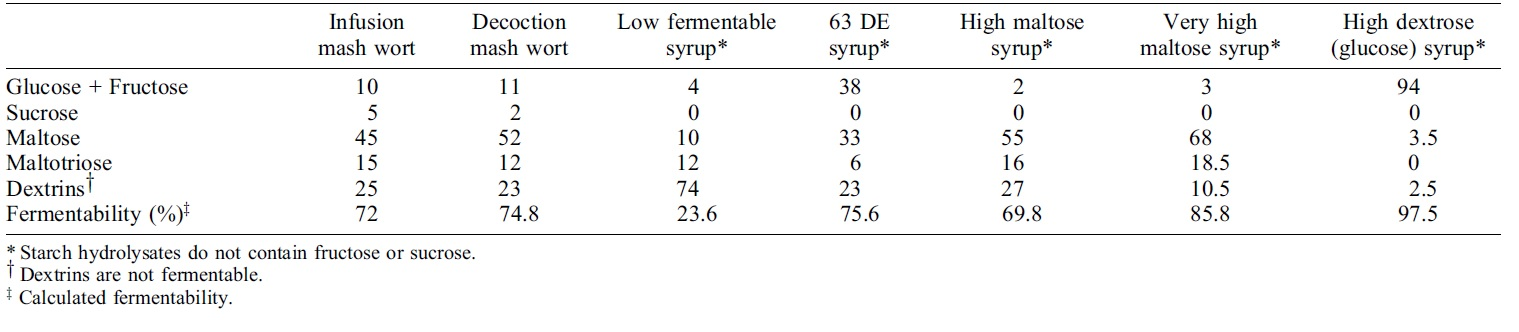
\includegraphics[width = \textwidth]{MashingTable}
\begin{table}[H]
	\caption{The carbohydrate compositions of two worts and several syrups prepared from starches ($\%$)\cite{Brewing_Science}}
\end{table}
\end{figure}

\section{Worting}
In favor of clarity, in the scope of this work I will define a step of the process which I will name "Worting". To the experienced, it is a combination of Lautering and secondary boiling.\\
After the mashing process is complete, the next step is to begin Worting the mash. Worting involves two main steps:\\
The first step consists of separating the grains from the mash. This is commonly achieved in large breweries by filtering the grains from the mash as it is being transferred into a secondary pot for the Worting process. Microbreweries sometimes preform the same action, however it is common to use only one pot, resulting in use of specialized bags or sieves to hold the grains during the mashing process, and removing them before Worting. At this stage, Hops (\textit{Humulus lupulus}) are added into the brewing mixture in order to add flavor and texture, as well as control the bitterness of the final product.\cite{Hops}\\
The second step of the process involves boiling the now grain-free mash to eliminate bacteria and sterilize the mixture - resulting in a sugary grain juice named Wort.

\pagebreak

\section{Fermentation}
After the Worting process is complete, the Wort is chilled to a predetermined temperature range which depends on the type of beer being brewed. The chilled wort is transferred into a new air sealed container where yeast of the genus \textit{Saccharomyces} are added to it at a common rate of $15-20 \cdot 10^6$ cells per m$L^{-1}$ - a process called Pitching. The yeast which are added to the Wort will consume the abundant sugars and convert them into ethanol and higher alcohols, all the while producing $CO_2$ as a byproduct. The yeast's action will, over time, transform the sugary grain juice into what is recognized as beer.\\
During this relatively long process which lasts from a few days up to several weeks, the most common way of measuring the progress of the fermentation process is via extracting a sample of wort by hand and measuring the liquid's specific gravity - the ratio between the density of the liquid and that of water measured at 4 $C^\circ$ - by dipping a hydrometer in the sample.\\
As fermenting beer is very sensitive to contamination and oxidization, this method of measurement, by far the most common one, is far from optimal. \cite{Biochemistry}

\section{Packing}
After the yeast have finished their work, the final step of the process is to package the beer in sterilized bottles or cans. In most microbreweries, the bottling is conducted by utilizing specialized tools to deliver the beer from the fermentation tanks to the bottles while limiting contact with the surrounding air as much as possible - contact with air at this step exposes the beer to severe contamination risk,  which endangers the products safety, and oxidation, which leads to considerable worsening of flavor and taste.\\
In most microbreweries it is common to add additional saccharides - most commonly white sugar or glucose syrup - to the bottled beer in order to stimulate additional fermentation after capping the bottles, ensuring sufficient carbonization of the final product.

\section{Reasons for this thesis}
As is now clear, the nature of the fermentation process as it is carried out in most microbreweries means it cannot be continuously or accurately measured, as every measurement of the fermentation process endangers the final products safety and taste. In addition, every measurement of the fermentation's progress wastes beer, as the retrieved sample cannot be returned to the fermenting mass.\\
In addition, accurate measurement of the fermentation process would allow early bottling of the beer, eliminating the need to add sugar or other saccharides to stimulate sufficient carbonization and assuring a healthier, tastier, and safer product.

\pagebreak

\begingroup
\renewcommand{\cleardoublepage}{}
\renewcommand{\clearpage}{}
\chapter{Fermentation Measurement Methods}
\endgroup

In this chapter, I will discuss the various methods used by different institutes and businesses to monitor the progression of Wort fermentation processes - most commonly by measuring in various ways its Ethanol content.\\
I will investigate five methods of Ethanol measurement:\\

\begin{itemize}
	\item Densitometry
	\item Near and Mid Infra-red Spectroscopy
	\item Gas Chromatography
	\item Hydrometry
\end{itemize}

In the following chapter, I will discuss the methodology of these five alternatives, as well as examine their use cases and feasibility for use in micro-brewing and large breweries alike.\\

\newpage

\section{Densitometry}
The first method of measuring ethanol in beer fermentation processes I will explore is utilizing a digital density meter.\\
As fermentation progresses, the yeast pitched into the Wort earlier will convert the saccharides into ethanol, higher alcohols, and carbon dioxide. This process eliminates the Worts sweetness, revealing the bitterness given by the hops, and transforming the Wort into beer. \\
While this process is not fully explored yet \cite{Brewing_Science}, it has a measurable effect on the Worts density, an effect which, while not linear, is pretty well understood and charted.\\
As the correlation between Worts density and alcohol content is well explored, it is possible to identify current alcohol content in a sample by identifying its density. Since finding out a liquids density is rather challenging, it is common to use a digital density meter\cite{Ethanol_Measurement}.\\

\begin{figure}[H]
	\centering
	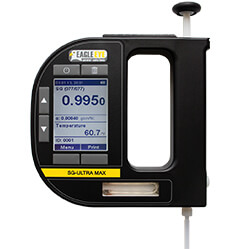
\includegraphics[scale = 0.6]{sg-ultra-max-digital-densitymeter-d}
	\caption{A SG digital density-meter}
\end{figure}

A digital density meter works by extracting a small sample of liquid, and injecting it into an oscillating U shaped tube. The tube is then piezoelectrically or electromagnetically excited into un-damped oscillation, vibrating two tubes - one with a sample, the other with a reference material. As the oscillating volume is known, it is possible to deduce its density from the period in which it oscillates based on the following relation:
\begin{equation}
	\tau = 2\pi \sqrt{\frac{\rho_sV_c+m_c}{\mathcal{K}}}
\end{equation}
Where $\rho_s$ is the density of the liquid to be discovered, $V_c$ is the internal volume of the u-tube, $m_c$ is the mass of an empty u-tube, and $\mathcal{K}$ is a manufacturer defined constant.\\

This method is mostly chosen due to its flexibility and reliability - substances will oscillate in different frequencies directly affected by their respective densities, and overfilling the device will not impact the measurement results\cite{Density_Measurement}.
\begin{figure}[H]
	\centering
	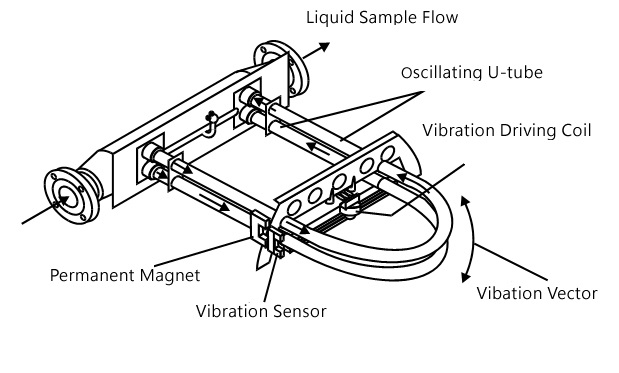
\includegraphics[scale = 0.45]{u-tube-density-meter}
	\caption{An example of a digital density meter working principle}
\end{figure}

While common in many industrial fields, a digital density meter is an expensive device. While it may be suitable for companies or research laboratories, it is not so fitting for private individuals.

\section{Near and Mid Infra-red Spectroscopy}
Near and Mid Infra-red Spectroscopy, respectively NIRS or MIRS, are twin methods which may be used for measuring ethanol content in liquids. To avoid repetitivity, I will explore how NIRS work, and detail the major differences between the methods.\\
NIRS is a spectroscopic method which utilizes electromagnetic radiation(EMR) from the near infrared region, typified by wavelengths of 700-1100 nm\cite{NIR_Spectroscopy_Ethanol}. In very broad strokes, Spectroscopy may be defined as studying the way in which different molecules react to EMR, and can be seen as the implementation of Beer-Lamberts law, which describes the relation between the attenuation of light to the properties of the material through which the light is traveling.\\
Since specific molecules diffract specific wavelengths, a samples composition may be understood and analyzed by studying which wavelengths of EMR are absorbed by it.

\begin{figure}[H]
	\centering
	\includegraphics[scale = 0.75]{spectrometer}
	\caption{NIRS DS2500 Analyzer by Metrohm NIRSystems}
\end{figure}

A spectrometer can be similarly defined as an instrument which illuminates a sample material with EMR of various wavelengths and measures the diffraction of electromagnetic radiation caused by the sample material.\\
Most spectrometers work by having a light source shine light through a prism or other light diffracting objects, such as specialized grates. The diffracted light is then filtered via a movable slit, allowing to select a specific wavelength range, which is then shined at a photo-diode or photo-transistor through the tested sample. The measured current generated by the photo-diode is then converted into a useful reading.

\begin{figure}[H]
	\centering
	\includegraphics[width = \textwidth]{spectrometer_scheme}
	\caption{Spectrometer operating principle}
\end{figure}

In our relevant case, a good correlation has been found between the presence of Ethanol molecules and the intensity of backscattered light at 905 $nm$  \cite{NIR_Spectroscopy_Ethanol}, allowing us to identify it in sample compounds.\\
MIR and NIR, being two different approaches to the same problem, are often used in conjunction for better results - NIR having greater sample penetrability and MIR suffering from less noise.
Until rather recently, NIRS instruments required sanitized environments, highly trained operators, and were generally quite large and bulky - making them more suitable for lab work rather than field work\cite{NIR_For_Spices}.\\ While in recent years more modern devices are being prototyped which will be smaller and can operate in a wider range of environments, using a spectrometer still requires specific training and experience, and a spectrometer is still an extremely expensive device.

\section{Gas Chromatography}
Gas Chromatography is a rather less common method of analysing beer, and is mostly used by research institutes and tax authorities, as it provides rather consistent reproducibility and works well with small samples.\\
Chromatography is an umbrella term for several methods following a common principle - different materials have different adsorption rates. Adsorption is the term given to the tendency of various atoms and molecules to stick to certain materials in differing rates. The adhesive properties of materials are determined experimentally for specific material-molecule pairs - for example, a 2004 study established that the saturation coverage of Ethanol on Silicon is 0.42 $\pm$ 0.10.\cite{Ehtnaol_adsorption,Gas_Chromatography_beer}\\

\begin{figure}[H]
	\centering
	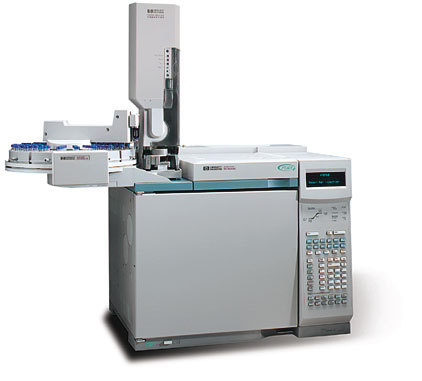
\includegraphics[scale = 0.4]{refurbished-gas_chromatograph}
	\caption{Gas Cromatograph (picture by BVK Technology Services)}
\end{figure}

When performing a gas chromatography test, a sample of beer is retrieved and injected into the gas chromatograph via a mechanical syringe. \\
The sample is evaporated and immediately mixed with an eluant - a neutral, non-reactive carrier gas, in most cases Helium. The Helium assists the gaseous mixture in travelling through the $column$, a thin metal or glass tube which houses a liquid with a high boiling point. \\
As the gaseous mixture travels through the heated tubing, it separates into its constituent parts. The samples components travel through the tubing in different velocities, until they are expelled through a detector at the end of the tubing, which varies by maker.

\begin{figure}[H]
	\centering
	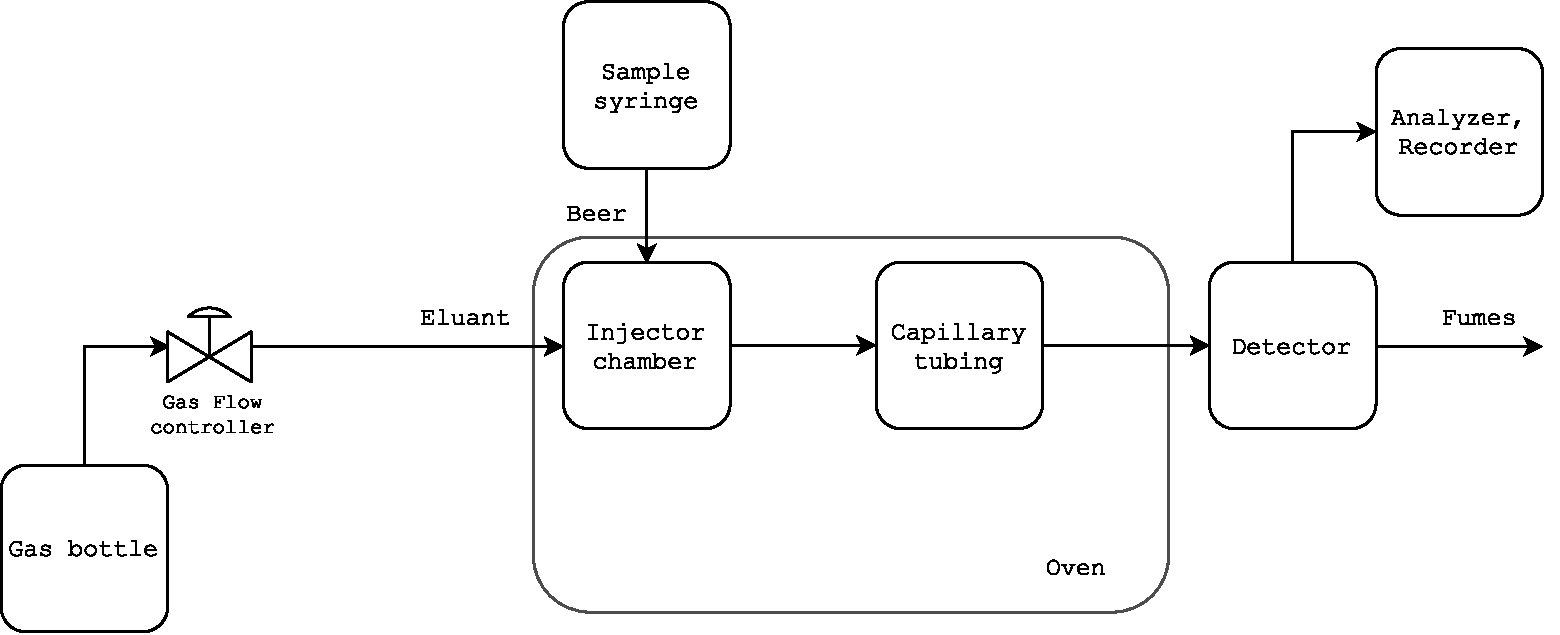
\includegraphics[width = \textwidth]{Gas_Chromatograph_PDF}
	\caption{Gas Cromatograph flow chart}
\end{figure}

Gas chromatography is highly complex and very expensive method which has little to offer for micro-breweries. While it is very precise and has high reproducibility potential, these are traits which are less important to the average micro-brewer. Therefore, it is almost never implemented within this context, except perhaps by those most pedantic about accuracy of results.

\newpage

\section{Hydrometry}
Hydrometry is the most common of all ethanol measurement techniques, as it is the cheapest and easiest to understand and utilize.\\
In the next chapter I will delve deeply into how a hydrometer works and why it was chosen as the cornerstone method of the physical implementation of this thesis.

\pagebreak

\begingroup
\renewcommand{\cleardoublepage}{}
\renewcommand{\clearpage}{}
\chapter{Solution proposition}
\endgroup

In this chapter I will discuss how hydrometry work and why it is the most common method for evaluating the amount of ethanol in fermenting beer, examine its greatest issue, and propose a solution for this risk.

\section{How Hydrometry work}
Hydrometry is simple, easy, and cheap to perform, and provides a sufficiently accurate measurement of ethanol contents.\\
Hydrometry can be viewed as an application of Archimedes principle: "Any object immersed in fluid, partially or wholly, is acted upon by a buoyant force equal to the weight of the fluid displaced by it". A hydrometer is a marked instrument, commonly made from glass and weighed by lead\cite{Ethanol_Measurement}, weighted so as to achieve neutral buoyancy, with the point on the hydrometer at water level while it is in buoyant equilibrium marked as the instruments baseline. The baseline is marked as $1.000$, to denote that there is no difference between the fluids density and that of water. Due to historical reasons, in Britain it is commonly marked up by three orders of magnitude, marking the baseline as $1000$\cite{Brewing_Science} instead of $1.000$\\
As the hydrometer floats around a certain equilibrium point in water, and its precise weight and volume is known, it is possible to deduce the sample fluids specific gravity - its density compared to that of water - based on the difference between the height of the current equilibrium point relative to that of water. In simpler terms, the denser the fluid, the higher the hydrometer will float in the fluid due to a stronger buoyant force acting on it.\\
The instrument is notched or marked in various distances to simplify reading its results, each notch indicating a different specific gravity. It is also calibrated around a specific temperature, in most cases 15 $C^{\circ}$\cite{Ethanol_Measurement}. As temperature has a noticeable effect on density, and as a result on specific gravity(SG), most charts detailing correlation between SG and hydrometer readings also correct for temperature differences.\\


\begin{figure}[H]
	\centering
	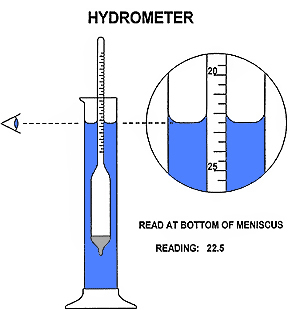
\includegraphics[scale=0.7]{hydrometer}
	\caption{Hydrometer operating principle \cite{Hydrometer_Pic}}
\end{figure}

In order to use a hydrometer, a sample of the Wort is retrieved after it has cooled to the desired temperature, but before the yeast has been pitched (see section 1.5). This reading will be designated as the Original Gravity(OG) of the batch being brewed, and all changes in the Worts SG due to an increase in ethanol content will be compared to this.

\section{The risk of Hydrometry}
To ensure accuracy, and to know when to proceed to the next stage of the brewing process, at least several measurements by hydrometer are required. However, every measurement involves retrieving a sample of fermenting Wort in order to measure its specific gravity.\\
Several solutions have been implemented to minimize exposure to contaminants and oxygen, which, at this stage of the process, can cause staling of the beer and severe damage to its taste and clarity. However, most of them are mechanical, and none of them has completely solved the issue.\\
Today, each micro-brewer must find their own point of balance between accuracy and risk, with each measurement increasing the accuracy of the process but endangering and expending the final product.



\section{Proposed solution}
Therefore, I propose eliminating the need to retrieve a sample of the fermenting beer altogether, and disposing of the last major risk factor in beer brewing.\\
The proposed solution will ensure a continuous - or, more accurately, discrete over very short intervals - measurement of the fermenting Worts SG, as well as calculate the current alcohol content while factoring in the environmental temperature. The device proposed will be integrated as a part of the closed fermenting Wort system, thus eliminating the danger of oxidation or contamination. Furthermore, it will allow wireless access to the results, so as to provide greater transparency of the brewing process.\\
The device will be a made from a Raspberry pi Zero W micro-computer connected to an HC-sr04 ultrasonic distance sensor and a DHT-11 temperature sensor - the exact architecture will be discussed at length in Chapter 4 of this work. The prototype designed and built for this thesis will be powered via cable, however future version may be battery operated. In order to ease integration and reduce costs, the device will utilize the hydrometer already present at every micro-brewery to complete the system. Should a micro-brewery not have a hydrometer, one may be supplied.\\

\begin{figure}[H]
	\centering
	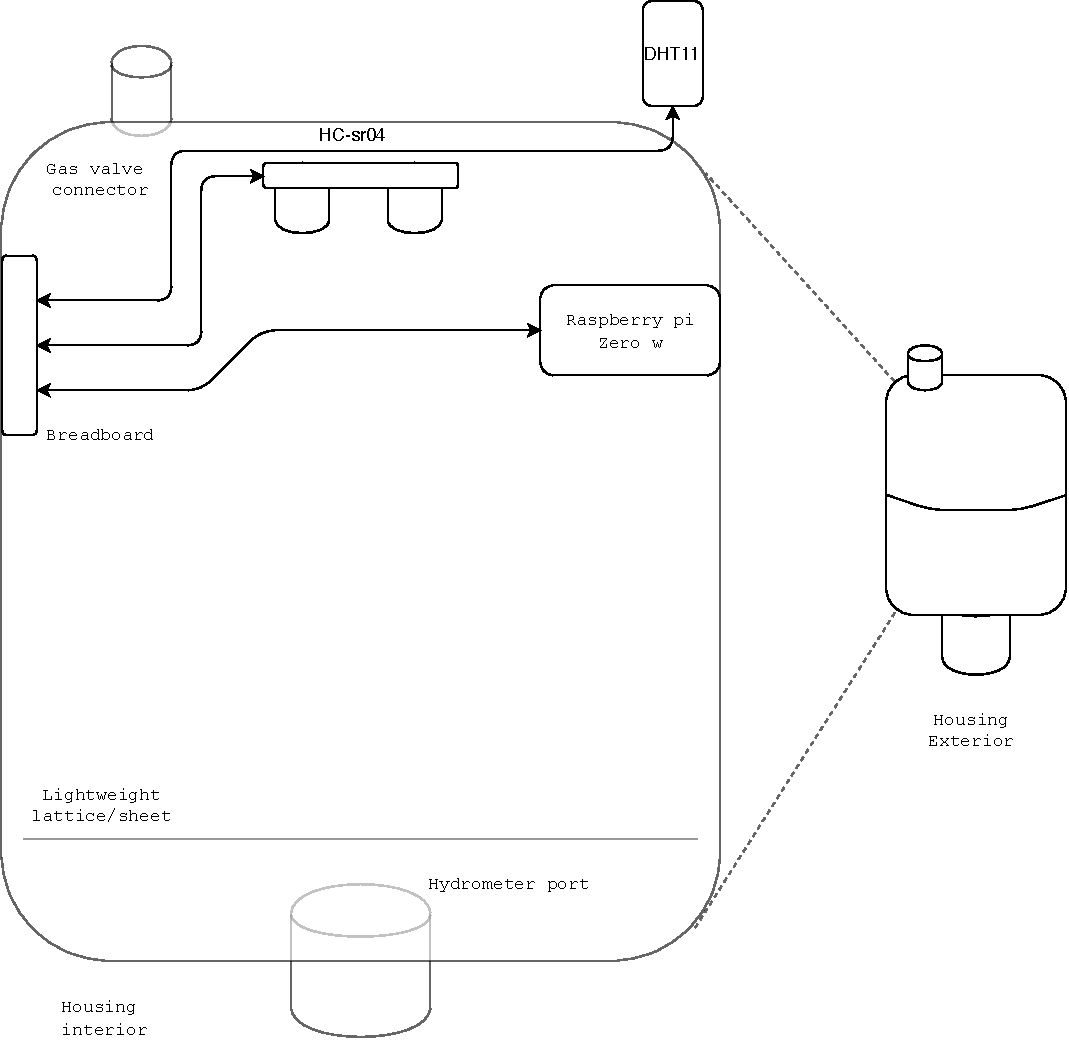
\includegraphics[scale=0.4]{Housing}
	\caption{General solution description}
\end{figure}

The final result will be a low cost, accurate, and reliable solution to provide insight into the process while eliminating the most common danger factors of traditional methods. In the next chapter I will elaborate on both the systems software and hardware architecture, as well as its implementation in the field.

\section{System Constraints}
Since the device relies on a hydrometer, there are several constraints which are imposed on the system due to it. In the scope of this work a relatively small - 19 cm - glass hydrometer is used. The hydrometer is marked in a range of 1.000-1.060 every 10 mm to denote a 0.010 change in the sampled liquids specific gravity(SG), with four additional smaller markings every 2 mm to mark differences of 0.002 between the larger marks.\\
These markings are marked along 60 mm of the hydrometers upper part. A hydrometer of this size and these markings is capable of measuring a total SG difference of 0.06, which correlates to a maximal difference in final alcohol content of 7.88$\%$ Alcohol By Volume(ABV). While it is possible to interpolate further into a wider range of measurements, the accuracy of measurement in the higher range of 7-10$\%$ ABV requires different calculations to remain accurate\cite{Joy_Of_Brewing}. As these beers are not common in micro-brewing, such additional calculations will remain as optional additions in the future.\\
Due to these limitations, the proposed device should be able to accurately identify changes of less than 2.0 mm, with a standard deviation of less than 0.5 mm, which translate into a 0.002 change in SG, or a 0.26$\%$ change in ABV. In this work I will aim for identification of a 1 mm difference, to provide a margin for inaccuracies due to environmental factors.


\pagebreak

\begingroup
\renewcommand{\cleardoublepage}{}
\renewcommand{\clearpage}{}
\chapter{Technical Implementation}
\endgroup

The devices design can be broken down into two parts: physical architecture and software architecture.\\
In this chapter, both of the architectures will be described, and their respective implementation discussed. The design schematics and pictures will be provided where relevant. Each part will be described, analysed, and justified where relevant.

\section{Physical Architecture}

The device will be mounted inside a custom housing which will hold all of the relevant components. These components are:

\begin{itemize}
	\item Raspberry Pi Zero W
	\item HC-sr04 Ultrasonic sensor
	\begin{itemize}
		\item 1,000 $\Omega$ resistor
		\item 2,000 $\Omega$ resistor
	\end{itemize}
	\item DHT-11 Digital Humidity and Temperature sensor
	\begin{itemize}
		\item 10,000 $\Omega$ resistor
	\end{itemize}
	\item Mini Breadboard
	\item Hydrometer
	\item Lattice/rice paper attachment
	\item Housing unit
\end{itemize}

With the exception of the lattice/paper attachment and the Housing unit, the estimated cost of parts for the entire project stands at 12.84 $USD$, or 264.61 $CZK$.\\
Next, I will examine and justify each component selection.

\subsection{Raspberry Pi Zero W}
The Raspberry Pi Zero W, henceforth RPi, is a low cost micro-computer, currently priced at 10$\$$ USD. The RPi is small, measuring only 0.065 mm x 0.030 mm x 0.005 mm in size, making it ideal for small device control. It also features a 1 GHz ARM11 processor, 512 MB of RAM, and a wireless LAN 2.4 GHz 802.11n surface-mount component etched into the board.\\
This device was chosen for its ease of use, availability, versatility, and low cost. It is fairly durable, and easily replaceable.

\begin{figure}[H]
	\centering
	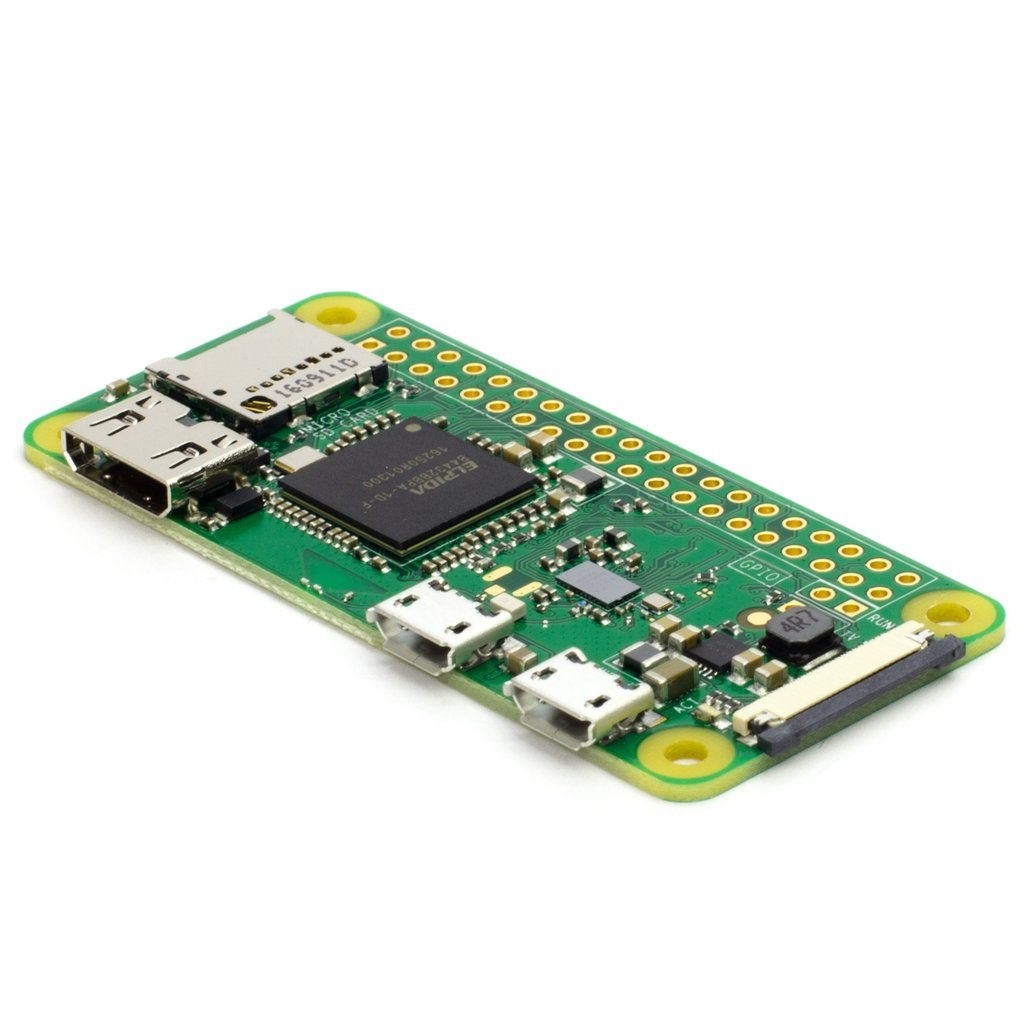
\includegraphics[scale=0.15]{RasPIZeroW}
	\caption{Raspberry Pi Zero W micro-computer \cite{RasPi0W}}
\end{figure}


\subsection{HC-sr04 Ultrasonic Ranging Module}
The HC-sr04 sensor provides a non-contact ultrasonic distance measurement function, at ranges of 2 to 400 cm $\pm$0.3 cm with a measuring angle of 30$^\circ$\\
The sensor works by emitting eight pulses at 40 kHz and listening for the rebounding pulses. It is then possible to computationally calculate, based on the length of the interval between the transmission and the reception of the rebounding signal, the distance between the sensor and the target.\\
The HC-sr04 sensor was chosen for this project due to it's high accuracy, small size, and low price. However, as the sensor's inherent inaccuracies may have a noticeable impact on such sensitive measurements, methods to compensate for them will be discussed and tested in Chapter 5.\\

\begin{figure}[H]
	\centering
	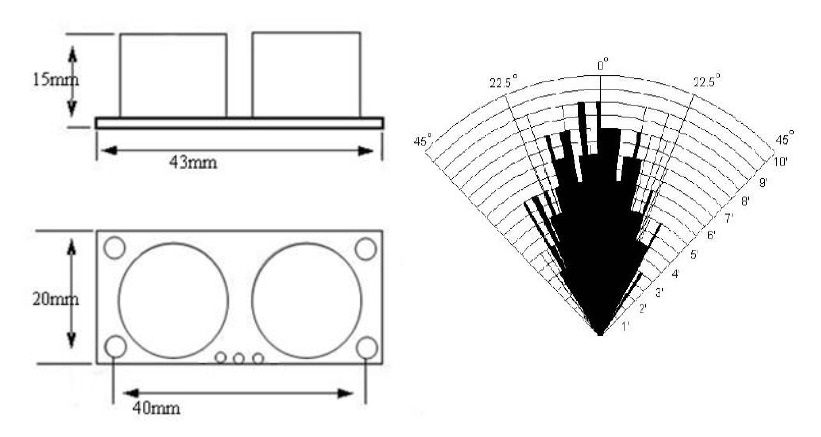
\includegraphics[scale=0.5]{HCSR04_sizes}
	\caption{HC-sr04 dimensions and angle accuracy \cite{HC-SR04}}
\end{figure}

As the sensor's output signal via the ECHO pin is rated at 5 V \cite{HC-SR04} and the Raspberry Pi's GPIO (General Purpose Input Output) is rated at 3.3 V\cite{RasPi0W}, it would be wise to implement some sort of protection for the board. The most effective way to provide such protection is a voltage divider, with the sensors output connected through it to the board. The values for the derivation of the required resistors can be found as follows:

\begin{gather}\nonumber
	\frac{V_{output}}{V_{in}} = \frac{R_2}{R_1 + R_2}\\\nonumber
	\frac{3.3}{5}= 0.66 = \frac{R_2}{R_1 + R_2}\\\nonumber
	0.66(R_1+R_2) = R2\\\nonumber
	0.66R_1 = 0.34R_2\\
	1.941R_1 = R_2
\end{gather}

Thanks to $(4.1)$, it is now clear that $R_2$ should have approximately twice the resistance of $R_1$. Therefore, in the scope of this device, the two chosen resistors were with resistances of 1000 $\Omega$ and 2000 $\Omega$, due to their abundance and price.


\subsection{DHT-11 Digital Humidity and Temperature sensor}
The DHT-11 Digital Humidity and Temperature utilizes a capacitive humidity sensor and a thermistor to measure relative ambient humidity with $\pm$5$\%$ accuracy at 25$^\circ$, and temperature with $\pm$2 C$^\circ$ at 25 C$^\circ$. The instruments readings are then digitalized via a built in microprocessor which transmits a digital reading from each sensor.

\begin{figure}[H]
	\centering
	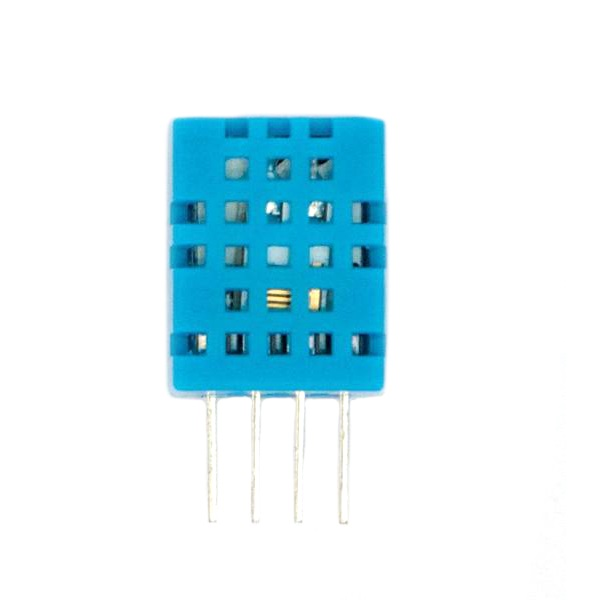
\includegraphics[scale=0.5]{DHT11}
	\caption{DHT-11 Digital Humidity and Temperature sensor\cite{HC-SR04}}
\end{figure}

A 10,000 $\Omega$ pull up resistor is placed between the power and data pins of the sensor to prevent it from over-heating and melting.

\subsection{Additional Components}
The rest of the components which are needed are generic and not type dependant: a mini breadboard, a hydrometer, several resistors, and a piece of paper. The housing unit can be a recycled bottle even, so while for the purposes of this work I will use a 3d printed one, any can be used in its stead.\\
\paragraph{Mini Breadboard} Is used to simplify prototyping - in a final product the various components will be soldered to each other, making a breadboard obsolete.
\paragraph{Hydrometer} Is a generic hydrometer - the specific gravity of the liquid is deduced by the change in the hydrometer height in wort compared to its height in water. Any hydrometer will do.
\paragraph{Resistors} Are used either as pull-up resistors or to form voltage dividers for the various sensors.
\paragraph{Lattice} Or a piece of rice paper act as a lightweight extension added on top of the hydrometer to ease its detection by the HC-sr04. This attachment is small and lightweight enough to make its addition to the system negligible.
\newpage
\section{Software Architecture}
The system will be coded entirely in Python to support modularity and ease of maintenance, supplemented by open-source software with appropriate licenses when necessary to assure high quality. The software architecture can be viewed as composed of several parts:\\

\begin{itemize}
	\item Raspbian Stretch
	\item Cron linux module
	\item Main software body
	\item Grafana
	\item InfluxDB
	\item Distance sensor thread
	\item Temperature sensor thread
\end{itemize}

Graphically, it may be viewed thus:

\begin{figure}[H]
	\centering
	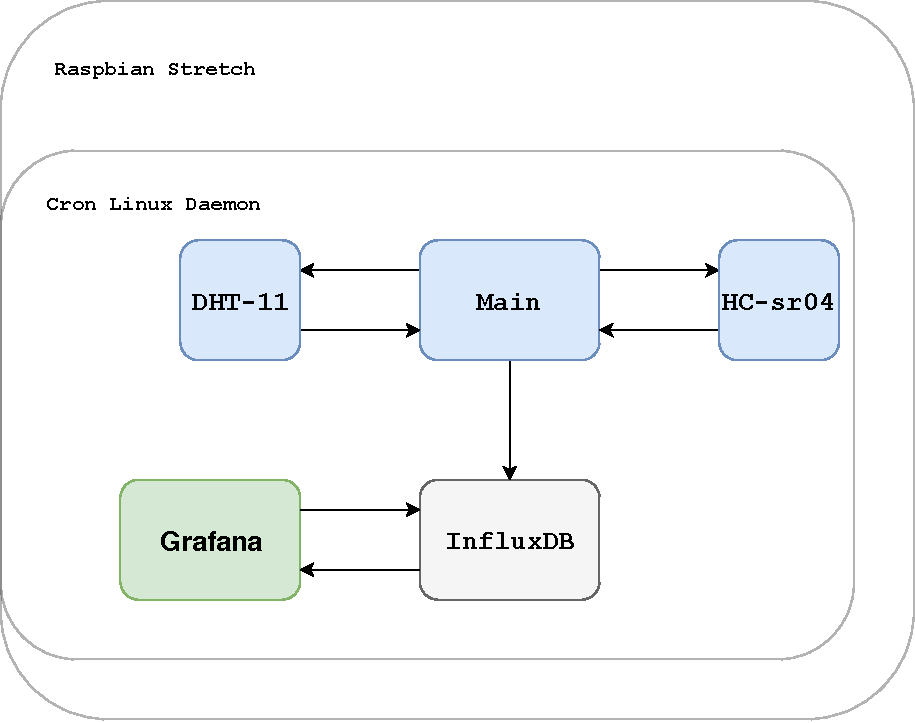
\includegraphics[width = \textwidth]{System_architecture}
	\caption{Software architecture flow chart}
\end{figure}

\subsection{Raspbian Stretch}
Raspbian Stretch is a Linux based operating system (OS) adapted for use with ARM processors. The version used in the scope of this work is that of April 2018, the latest in a long line of modifications made to the basic Raspbian system at the time of writing.\\
It was chosen as it is an OS specifically built to work well with Raspberry Pi's and their unique hardware.

\subsection{Cron Linux Daemon}
Cron, named after the Greek word for time, is a Linux Daemon - a program which runs in the background of an operating system as a process independent from user interaction. Cron, specifically, is a Daemon which assists in scheduling tasks, as it runs automatically once a minute based on the systems clock. It will be used to activate the Main software module automatically as the system boots, re-trigger it once a minute, as well as following and monitoring additional threads and processes created by the Main module.

\subsection{InfluxDB}
InfluxDB is an open source, time series database - meaning, it is a database optimized to handle data indexed by time. It support a unique SQL-like language with many time-centric built in functions. It can store data as 64 bit integers, floating points, strings, and booleans.\\
For this work, data will be stored in it entirely as a string data type.

\subsection{Grafana}
Grafana is an open source graph generating web server. It is capable of retrieving time series data and adding them seamlessly to graphs hosted locally on the machine it operates on.\\
It was chosen as a complement to InfluxDB due to the pair's great integration, as well as Grafana's flexibility and streamlined user interface.

\subsection{Main Software module}
The main software module (Main) holds the majority of custom function and process calls of the project. It is the part in charge of turning on or off the various sensor modules, as well as run three major calculations: convert the average distance measured by the distance sensor to a specific gravity (SG) reading as is measured by the hydrometer, correct SG based on temperature reading, and convert the corrected SG to alcohol percentages. The finalized, temperature compensated alcohol measurement will then be stored in InfluxDB for use by Grafana as a String data type.

\paragraph{Distance to specific gravity:}
A hydrometer reading correlates directly to its depth in liquid, i.e. its distance from the sensor. Due to the casing which holds the device, the sensors distance from the surface of the liquid is given at 18 cm. As said casing is to be submerged in liquid up to 2 cm, the hydrometers height above the water during minimal measurement (1.000, the SG of water) is 2.5 cm. Since the sensor height is 1.5 cm, the active measurement range is 12 cm. The hydrometer used for this work ranges in SG values between 1.000 to 1.060 across 6 cm.\\
These two parameters - distance from the sensor and SG reading - can be viewed as a Cartesian tuple. Therefore, as the relation between the two is linear, it can be derived with simple linear approximation:
\begin{equation}
y-y_1 = \frac{y_2 - y_1}{x_2 - x_1}(x - x_1)
\end{equation}

Which, in the scope of this work, will yield the following linear equation:

\begin{equation}
	y = 1.12 - 0.01 x
\end{equation}

Where $y$ is the SG and $x$ is the distance measured.\\

\paragraph{Specific gravity correction with relation to temperature:}
Since SG readings depend heavily on temperature, they have been traditionally corrected via tables correlating temperatures by degrees to values. Though it has been known for a while that the dependency of SG on temperature is linear \cite{Temp_To_SG}, a partial correlation factor was only proposed in 2003 \cite{Joy_Of_Brewing}:

\begin{equation}
C_p = 1.313454 - (0.132674\cdot f) + (0.00205779 \cdot f^2) - (0.000002627634 \cdot f^3)
\end{equation}

Where $C_p$ is the resultant partial correction factor and $f$ is the temperature in Fahrenheit at the time of measurement.\\
However, this relation assumes a hydrometer calibrated to older American standards at 59 f$^\circ$. Since modern hydrometers can sometimes be calibrated at 20 C$^\circ$, or 68 f$^\circ$, a corrected, complete, temperature independent relation has been proposed:

\begin{equation}
C_g = SG \cdot \frac{\splitfrac{1.00130346 - 1.34722124*10^{-4} \cdot f + }{2.04052596*10^{-6} \cdot f^2 - 2.32820948*10^{-9} \cdot f^3} }{\splitfrac{1.00130346 - 1.34722124*10^{-4} \cdot h_{ct} +}{ 2.04052596*10^{-6} \cdot h_{ct}^2 - 2.32820948*10^{-9} \cdot h_{ct}^3}}
\end{equation}

Where $C_g$ is the final corrected gravity, $SG$ is the measured specific gravity, $f$ is the temperature in Fahrenheit, and $h_{ct}$ is the hydrometers calibration temperature.\\

\paragraph{Corrected Gravity to ABV}

Once the finalized SG value is obtained, it is possible to employ an adapted version of the standardized polynomial for alcohol percentage by weight from original gravity (OG) measurements proposed by Neville and Hashemi\cite{PH_in_yeast}:

% Optional:
\begin{equation}
ABW = 76.08 \cdot \frac{OG - SG}{1.775-OG}
\end{equation}

Where OG is the original gravity, i.e the first specific gravity measured just before adding the yeast, and SG is the current reading.
The resulting Alcohol By Weight (ABW) percentage may then be converted into Alcohol By Volume (ABV), the more common unit of alcohol measurement in micro-breweries, as follows \cite{Brewing_Science}:

\begin{equation}
	ABV = \frac{A_{\%} \cdot C_g}{0.791}
\end{equation}

The Main module is switched on once a minute by Cron, and checks if the module is currently in operation. If it is, it will terminate and check again in the next Cron cycle. If not, it will start to collect the sensors measurements, process their results, and store them in InfluxDB as a finalized ABV value, from where Grafana will retrieve and display the finalized results.

\subsection{Hc-SR04 ultrasonic sensor module}
The sensor module interfaces with the HC-sr04 sensor and outputs an averaged output to improve the sensor's accuracy.\\
The sensor responds to a 10 $\mu$s pulse from the Raspberry Pi's General Purpose Input Output (GPIO) pins by emitting eight ultrasonic bursts at a frequency of 40 kHz and turning its output pin, named ECHO, to high until the sensor detects the returning ultrasonic burst. The sensor module logs the time stamp of the leaving pulse and the returning pulse to and compares them to identify $\Delta t$, which is how much time elapsed until the returning pulse was detected.\\

Since the pulse is travelling through air, it is safe to assume a constant and known speed of sound. as $v_{sound}$ is known and $\Delta t$ is measured, calculating distance $x$ is rather simple:

\begin{gather} \nonumber
v_{sound} = \frac{x}{\frac{\Delta t}{2}}\\
x = \frac{v_{sound}}{2}\cdot \Delta t
\end{gather}

As is known in literature, however, the speed of sound depend on the medium through which it travels. In air, the effect of humidity is negligible, while the effect of pressure is not\cite{Sound}. However, in the scope of this work, I will assume this device would not be used under pressure differing from 1 Atmosphere, or 101325 Pa.\\
Once the HC-sr04 module is awoken by the Main Module, it will conduct 26 measurements, as it needs to stabilize for 2 seconds between measurements to allow for higher accuracy. The average result of these measurements will then be sent back to the Main Module to be processed. The reason for choosing 26 measurements was to assure the process would last less than a minute to match with the work of Cron, but in Chapter 5 our physical experiments suggest a different number of measurements would be better. The different amount of measurements will be justified via experimental data.


\subsection{DHT- 11}
The way the DHT-11 sensor measures temperature and humidity is not revealed by its manufacturers, only how it receives and transmits data. Once the DHT-11 module is awakened by the Main Module, it will conduct 10 temperature and humidity measurements and output the average of the results back to the Main Module.

\newpage

\pagebreak

\begingroup
\renewcommand{\cleardoublepage}{}
\renewcommand{\clearpage}{}
\chapter{Testing}
\endgroup
In this chapter the testing process of the device will be discussed. In order to assure maximal accuracy and optimal usability of the device, this chapter will deal with three major tests. The first will be to test the distance sensor itself to assure that it is sufficiently accurate for our purposes. The second test would examine how many measurements would be sufficient to assure the accuracy of the measurement. The third test would be a complete test of the system, to verify its measurement capabilities.

\section{Hc-sr04 verification}
An experiment can be conducted in order to assure the ultrasonic distance sensor is sufficiently accurate.\\
For this work, the experiments equipment was a custom metal rig with a movable slide, a screen which shows the current measurement value, and an infra-red distance sensor with an absolute error of $\pm1\cdot10^{-4}$ mm which is used to measure the distance displayed.\\
The experiments procedure involved mounting the sensor on a the custom rig at a set point. A small object was placed on the custom rigs slide, which was moved to a random distance that was defined as zero, or the experiments starting point. From there the object was moved towards the sensor in 20 discrete steps of 1 mm each, to provide 20 measurements. A python routine was implemented to measure the distance to the object 26 times, and return the average of these measurements as well as their standard deviation. The measurement results can be seen in Table 5.1:


\begin{table}[H]
\centering
	\begin{tabular}{| c |c| c |}
		\hline
		Slide Movement cm & Distance Measured cm & Standard Deviation cm\\ \hline
		0 & 13.8086 & 0.277\\
		-0.1 & 13.637 & 0.269\\
		-0.2 & 13.6499 & 0.243\\
		-0.3 & 13.3111 & 0.146\\
		-0.4 & 13.2449 & 0.261\\
		-0.5 & 13.1002 & 0.116\\
		-0.6 & 13.0287 & 0.101\\
		-0.7 & 12.8443 & 0.385\\
		-0.8 & 12.8574 & 0.154\\
		-0.9 & 12.8026 & 0.212\\
		-1.0 & 12.6897 & 0.277\\
		-1.1 & 12.5778 & 0.139\\
		-1.2 & 12.4317 & 0.107\\
		-1.3 & 12.3913 & 0.129\\
		-1.4 & 12.1836 & 0.078\\
		-1.5 & 12.1268 & 0.122\\
		-1.6 & 12.0269 & 0.107\\
		-1.7 & 11.8908 & 0.114\\
		-1.8 & 11.9059 & 0.106\\
		-1.9 & 11.7074 & 0.095\\
		-2.0 & 11.6694 & 0.131\\
		\hline
	\end{tabular}
	\caption{Measurement results for distance sensors accuracy}
\end{table}



\begin{figure}[H]
	\centering
	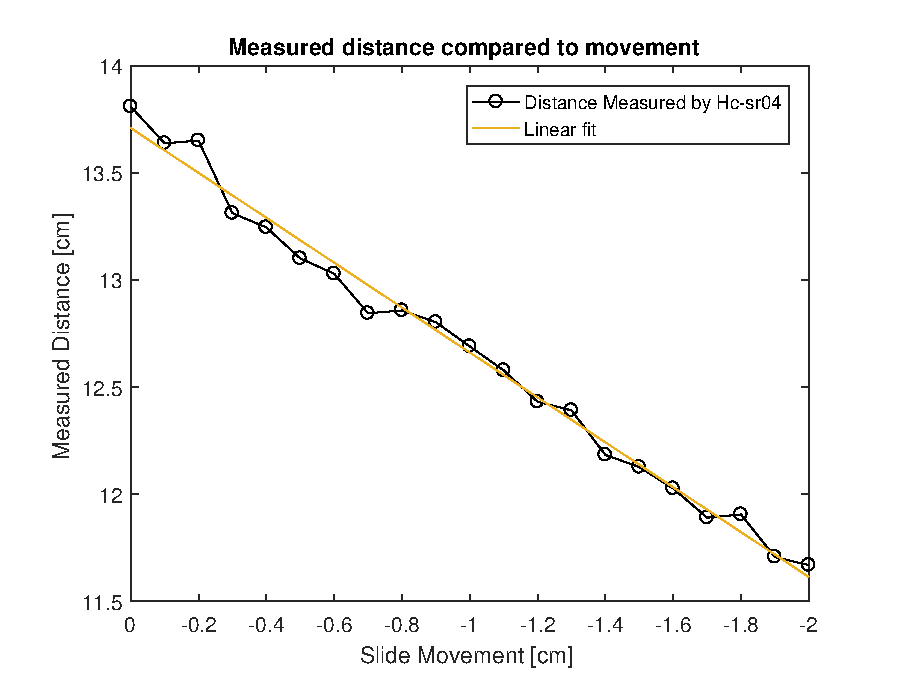
\includegraphics[width = \textwidth]{DistanceMeasuringGraphAndFit2}
	\caption{Measured distance compared to linear prediction}
\end{figure}

Note that as the slide was moving towards the sensor, its movement is noted as negative.
It is easy to see that the sensor preforms rather well despite its low cost, with an acceptable variation in the measurement result.\\
The sensor provides a fairly accurate measurement, which, over time, provides a rather linear relation, proving that with sufficient measurements the sensor can provide the necessary accuracy of less than 2 mm.

\section{Amount of measurements}
The sensors sensitivity in the previous section is entirely dependent on the averaged result of twenty six measurements taken in quick succession.\\
The original amount of measurements to be averaged was a compromise arrived at due to the sensors settling time - a two seconds pause between consecutive - and the one minute time limit imposed by Cron, encouraging the system to provide a data point every minute. However, since fermentation is a slow process which lasts at least a week\cite{Joy_Of_Brewing}, it is possible to perhaps waive the need to update the data every minute if the accuracy justifies it. As time is no longer such a pressing issue, it has been decided to update the database, and with it, the graphs and content, once every five minutes or less.\\
To discover the effect of the number of consecutive measurements taken on the accuracy of the result, the same rig which was used in the last measurement was used once more, only this time with a different purpose in mind: fifteen measurements were taken, with the slide moving one millimeter towards the sensor between each measurement cycle. During each cycle the sensor took more than a hundred distance measurements which validity was verified via calculating the standard deviation of each cycle automatically.\\
Then, after at least a hundred valid measurements of each distance were obtained, a program was created to calculate the standard deviation of various chunks of the measurement and see how the amount of measurements taken influence the standard deviation of the result. The program calculated the standard deviation of ten cross sections of the data (the first 10 readings, 20, 30, and so forth until 100 readings) across the 15 different distance measurements.\\
Five selected measurements out of the 15 different measured positions, the standard deviations of the first 10, 30, 50, 70, and 100 readings from each measurement, may be viewed below:

\begin{figure}[H]
	\centering
	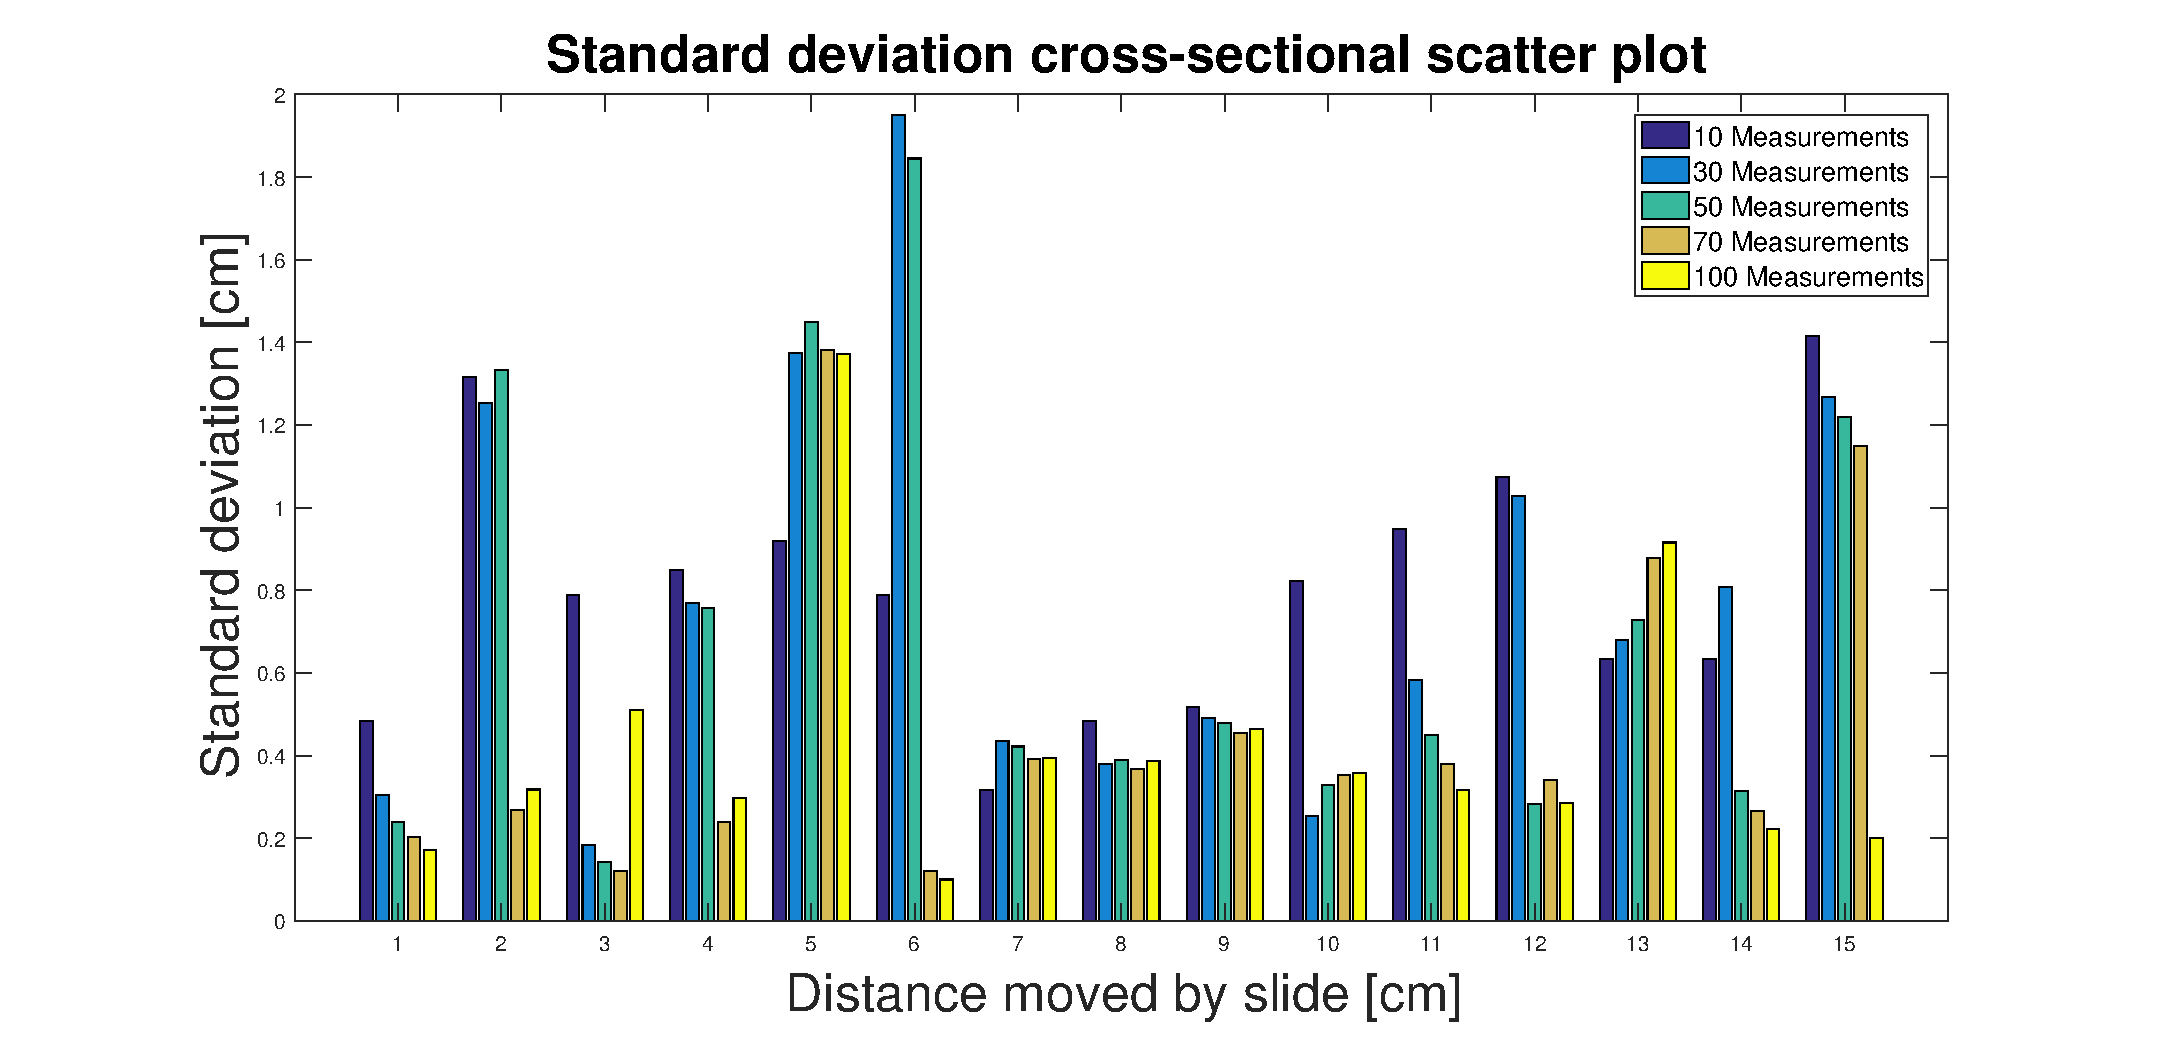
\includegraphics[width = \textwidth]{CrossSectionStdBars}
	\caption{Standard deviation cross section results from each measurement}
\end{figure}

\begin{figure}[H]
	\centering
	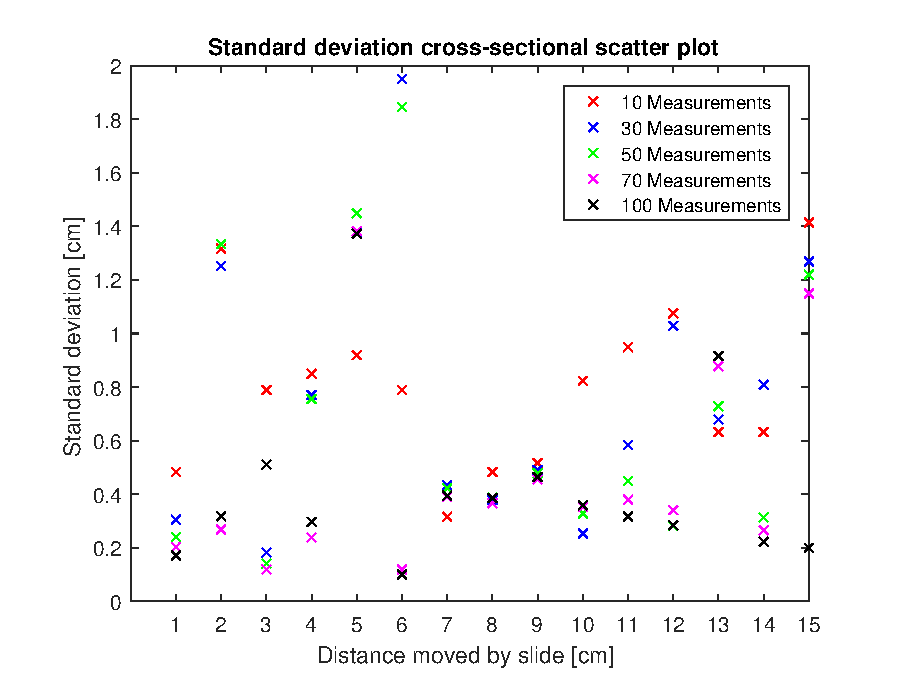
\includegraphics[width = \textwidth]{stdAcrossAllMeasurements}
	\caption{Standard deviation results as scatter plot}
\end{figure}



Since the results are very hectic and seemingly without a pattern, the standard deviation of each cross section of the measurements was recalculated to see how the number of readings taken affect the outcome and provide a far clearer result:

\begin{figure}[H]
	\centering
	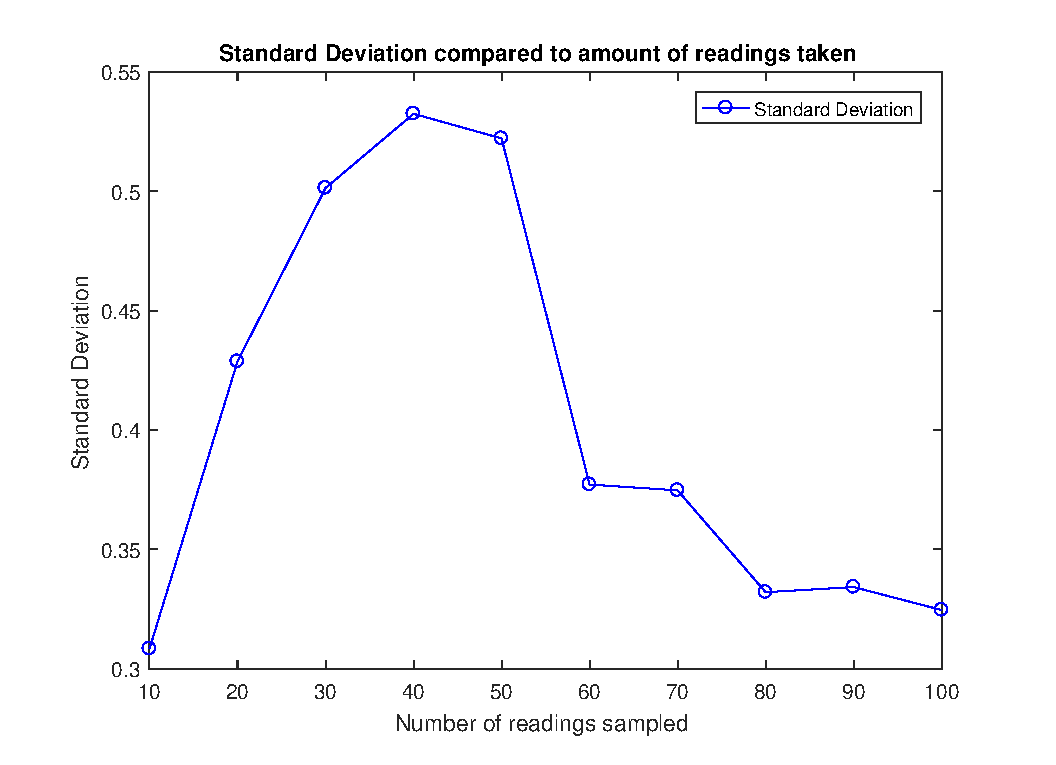
\includegraphics[width = \textwidth]{CrossSectionReadingsStd}
	\caption{Standard deviation of individual cross sections}
\end{figure}


As it is possible to see from the graph, the best results are the 10 readings per measurement and more than 80. Since 10 readings are not statistically valid - i.e. the low result is most likely a statistical fluke - and are far more vulnerable to environmental noise and bad readings than the higher values, it is safe to disqualify it as a viable solution. Since 100 readings take $202.54 s\pm0.00327$ as measured by a timer while being the least vulnerable to disturbances among the measured cross sections, it will be selected as the proper amount of readings for our system, balancing accuracy with time.
Therefor, for the optimal operation of the system, the distance from the sensor to the hydrometer will be sampled 100 times per cycle of the distance sensor module, with the average result being passed on for processing in the Main Module along with the temperature results from the DHT11 module.

\section{Verification of system capabilities}
After proving that the sensor is up to the task and adjusting the amount of measurements for optimal results, this section will deal with a simulated measurement of the entire device.\\
For this experiment, six solutions of water and sugar were created with a SG value of 1.005, 1.010, 1.015, 1.030, 1.040, and a control solution of pure water at 1.000. Since there is no way to fully simulate the heat generated by fermentation in a tank to be measured by the temperature sensor, all the liquids were kept at a control temperature of 20 $C^\circ$ matching the hydrometers calibration temperature.\\
The set up involved placing the Hc-sr04 sensor at a distance of 14.5 cm from the surface of the solution, to simulate the distance granted by the housing unit.
A hydrometer was placed in each solution, with a negligibly light piece of paper, weighing 0.008 grams, on its edge to assure accurate reading by the distance sensor. The hydrometers depth in each solution was measured by the systems standard of the average of 100 distance readings, which was then fed into the Main Module for the conversion to SG.\\
The result of the measurement were:

\begin{table}[H]
	\centering
	\begin{tabular}{| c |c| c |}
		\hline
		Solution SG & Measured SG & Standard Deviation\\ \hline
		0 & 1.001 & 0.0020\\
		1.005 & 1.007 & 0.0022\\
		1.010 & 1.009 & 0.0010\\
		1.015 & 1.015 & 0.0032\\
		1.030 & 1.029 & 0.0028\\
		1.040 & 1.041 & 0.0018\\
		\hline
	\end{tabular}
	\caption{Measurement results for system capabilities}
\end{table}

\begin{figure}[H]
	\centering
	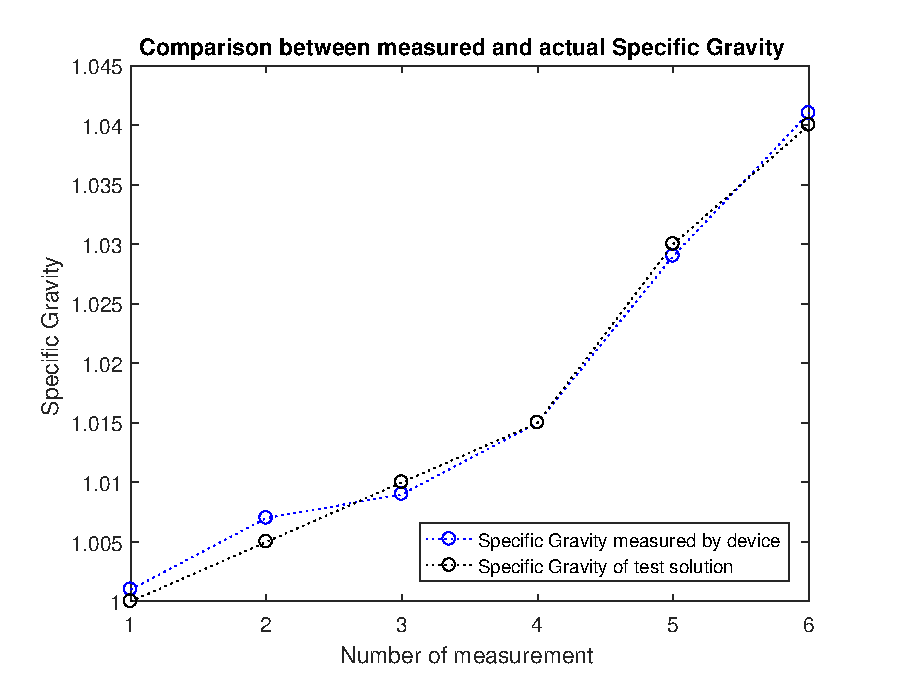
\includegraphics[width = \textwidth]{SpecificGravityComparison}
	\caption{Comparison between measured and actual specific gravity}
\end{figure}

\begin{figure}[H]
	\centering
	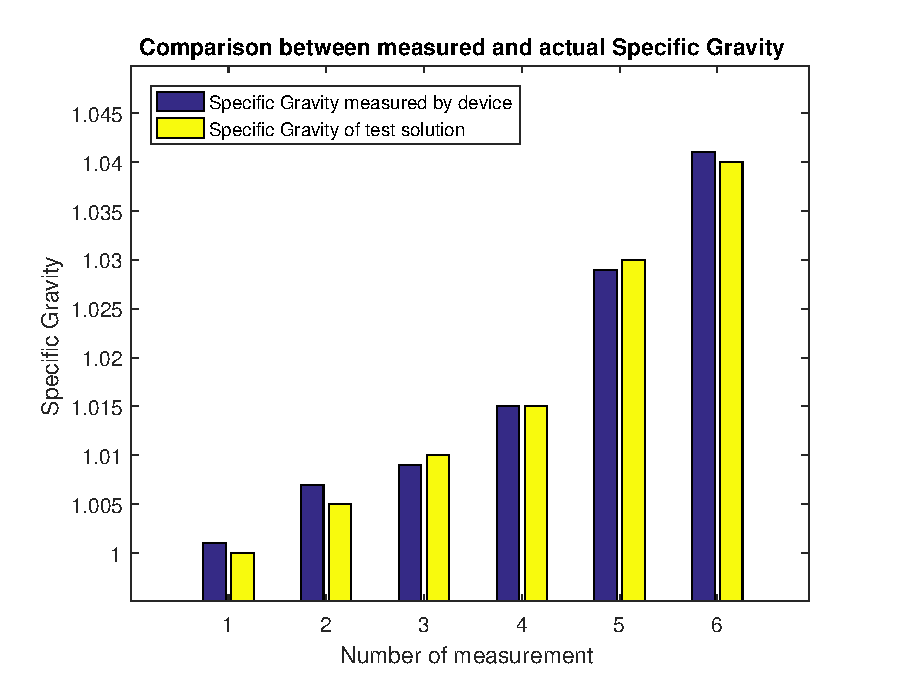
\includegraphics[width = \textwidth]{ComparisonBars}
	\caption{Bar graph of measured and actual specific gravity}
\end{figure}

As can be gleaned from the experiments, the system can match the actual specific gravity to within 0.002, and over time could probably achieve a better result.


\pagebreak

\begingroup
\renewcommand{\cleardoublepage}{}
\renewcommand{\clearpage}{}
\chapter{Discussion and Conclusion}
\endgroup
This chapter will be dedicated to the discussion of this works results, the business case for the designed and prototyped device, how can it be improved in the future, as well as the conclusion of this thesis.

\section{Discussion}
The tests conducted in Chapter 5 proved sufficient to determine the accuracy of the HC-sr04 sensor and its appropriateness for use in this device.	The experiments conducted show that, a few measurement errors aside, the sensors accuracy is 2 mm or less when 26 measurements are taken and the optimal number of readings to be implemented are 100.\\
It is worth noting, however, that the temperature readings could not be accurately recreated without an active beer fermentation process. While the maximal difference in temperature between the fermenting wort and the air above it is expected to be less than one degree Celsius\cite{Thermodynamics_Brewers}, it merits further examination. Despite this, it is clear from the experiments conducted that the device preforms as predicted, and sometimes even better.\\
This prototype was built as an expandable platform, designed to accommodate future add ons to both hardware and software. Additional software modifications could include a calibration function to allow for the sensor to be used with all types of hydrometers, breweries, and brews; curve fitting to predict when the fermentation would end or when it is best to end it; Google Weather integration to better understand the impact of environmental factors on fermentation; and IoT architecture integration, to implement better fermentation predictions based on data gathered from several such devices, as well as study seemingly unrelated disturbances and their effects on beer brewing.\\
Hardware additions could be different sensors to provide extended functionality, better connectivity, or improve the service provided by this device, as well as battery to eliminate the need for constant connection to power.

\pagebreak

\section{Business proposal}
The device targets the very niche market of micro-brewing, which luckily narrows the target audience immensely. A possible marketing strategy would be to propose a modular model of the device, so that every possible type of customer can enjoy their preferred version.\\
Due to the low cost of the device it is possible to offer the most basic version of it for at least a 300$\%$ markup, and offer several varieties - for example assembled, disassembled, with 3D printed housing, etc.\\
I believe previous attempts at this market have have failed due to the competing products being extremely expensive, or being so complex that they required specific training and immense previous knowledge.\\
A possible marketing strategy could involve ads in targeted literature, as well as a crowd-funding campaign as both a way to gather an initial cash reserve to fund assembly and a marketing push. As most of the micro-brewing market do so as a hobby, suggesting this as a low-cost "Do it yourself" device which can be assembled by the clients themselves would increase product interaction, as well as seem as an addition to their current brewing process and personal skills.

\section{Conclusion}
The aim of this thesis work was to design and build a low cost, high accuracy device to monitor the progression of beer fermentation processes. The proposed device was to be accurate enough to be useful, and yet cheap enough that small, private micro-breweries would benefit from using it.\\
The proposed device was assembled in its entirety, with the exception of the housing unit, for less than 13$\$$US, or 283.28 $CZK$. The total cost of device assembly was about 3.25$\%$ of its mechanically closest competitor, BrewGuard, a 400$\$$US device which failed due to its high price. As proven in Chapter 5, the device can reach an accuracy of 1 mm, and provide an accurate measurement of Alcohol By Volume.\\
It matched out initial parameters, with a distance measurement accuracy of less than 2 mm and a deviation of less than 0.002 specific gravity.\\
Unlike current market solutions, the device could be utilized by almost anyone with minimal instructions and enable greater insight into the fermentation process - allowing for vastly superior customizability and predictability of the resulting beer.\\
To conclude, this device was designed, programmed, and built using the diverse knowledge learned during my time in Czech Technical University, and drew upon know-how taught in the many courses in the Robotics and Cybernetics program - from calculus and physics to databases and networks - with the result being an accurate, low cost, easy to deploy in situ measuring device.



\appendix

\begin{thebibliography}{9}
	\bibitem{Brewing_Science}
	\textit{\textbf{Brewing Science and Practice}}\\
	D. E. Briggs ; C. A. Boulton ; P. A. Brooks ; R. Stevens\\
	Woodhead Publishing Limited and CRC Press LLC, 2004

	\bibitem{Brewing}
	\textit{\textbf{Brewing}}\\
	M. J. Lewis ; T. W. Young\\
	Springer Science \& Business Media\\
	\textit{6.12.2012}\\
	ISBN 9780306472749

	\bibitem{Malting_Brewing}
	\textit{\textbf{Malting and Brewing Science: Volume II Hopped Wort and Beer}}\\
	J. S. Hough ; D. E. Briggs ; R. Stevens ; T. W. Young\\
	Springer Science \& Business Media\\
	ISBN 978-1-4613-5727-8

	\bibitem{Malting}
	\textit{“Effect of Malting Temperature and Mashing Methods on Sorghum Wort Composition and Beer Flavour.”} \\
	M. A. Igyor, et al. \\
	\textit{Process Biochemistry}, vol. 36, no. 11, 2001, pp. 1039–1044.\\
	doi:10.1016/s0032-9592(00)00267-3.

	\bibitem{Hops}
	\textit{“125th Anniversary Review: The Role of Hops in Brewing”}\\
	C. Schonberger ; T. Kostelecky\\
	\textit{Journal of the Institute of Brewing}, vol. 117, no. 3, 2001, pp. 259-267.\\
	doi:10.1002/j.2050-0416.2011.tb00471.x

	\bibitem{Biochemistry}
	\textit{\textbf{Biochemistry of Beer Fermentation}}\\
	E. Pires ; T. Branyik \\
	Springer international publishing\\
	ISBN: 978-3-319-15188-5

	\bibitem{Ethanol_Measurement}
	\textit{“Evaluation of Ethanol Measuring Tehcniques”}\\
	S. Hennessey ; K. Payne\\
	\textit{Worcester Polytechnic Institute}, 2015\\

	\bibitem{Density_Measurement}
	\textit{"Density Measurement using modern oscillating transducers"}\\
	H. Stabinger\\
	\textit{South Yorkshire Trading Standards Unit}, 1994

	\bibitem{Nondestructive_Measurement}
	\textit{\textbf{Nondestructive Evaluation of Food Quality Theory and Practice}}\\
	S. N. Jha, et al.\\
	Springer Science \& Business Media\\
	ISBN 978-3-642-15795-0

	\bibitem{NIR_For_Spices}
	\textit{"Comparison of Near-and Mid-Infrared Spectroscopy for Herb and Spice Authenticity Analysis"}\\
	K. Lawson-Wood ; I. Robertson ; U. K. Seer Green\\
	\textit{PerkinElmer, Inc.}, 2016

	\bibitem{NIR_Spectroscopy_Ethanol}
	\textit{"Noninvasive Method for Monitoring Ethanol in Fermentation Processes Using Fiber-optic Near-Infrared Spectroscopy"}\\
	A. G. Cavinato ; D. M. Mayes ; Z. Ge ; J. B. Callis\\
	\textit{Analytical chemistry 62, no. 18: 1977-1982}, 1990

	\bibitem{Gas_Chromatography_beer}
	\textit{"A rapid method for determination of ethanol in alcoholic beverages using capillary gas chromatography"}\\
	M. L. Wang; Y. M. Choong ; N. W. Su ; M. H. Lee\\
	\textit{Journal of Food and Drug Analysis, 11(2)}, 2003

	\bibitem{Ehtnaol_adsorption}
	\textit{"Adsorption of ethanol on Si (1 0 0) from first principles calculations"}\\
	P. L. Silvestrelli\\
	\textit{Surface science, 552(1-3), 17-26}, 2004

	\bibitem{Ethanol_in_Wine_GC}
	\textit{"Quantitative determination of ethanol in wine by gas chromatography"}\\
	B. Stackler ; E. N. Christensen(1974)\\
	\textit{American Journal of Enology and Viticulture, 25(4), 202-207.}

	\bibitem{Hydrometer_Pic}
	\textit{"Racking the Hard Cider"}\\
	\textit{http://www.windward.org/notes/notes70/andrew7010.htm}\\
	Accessed on 26.3.2018

	\bibitem{HC-SR04}
	\textit{"Product User’s Manual – HCSR04 Ultrasonic Sensor"}\\
	Cytron Technologies Sdn. Bhd.

	\bibitem{RasPi0W}
	\textit{Pimoroni Tech Store}
	\textit{"https://shop.pimoroni.com/products/raspberry-pi-zero-w"}

	\bibitem{DHT11}
	\textit{Temperature and humidity module DHT11 Product Manual
		www.aosong.}\\
	Aosong(Guangzhou) Electronics Co.,Ltd

	\bibitem{Temp_To_SG}
	\textit{"EFFECT OF TEMPERATURE ON THE SPECIFIC GRAVITY OF WORT"}\\
	L. H. Hawkins; P. E. Gough\\
	\textit{Brewing industry research foundation, Vol 69, 139-141, 1963}

	\bibitem{Joy_Of_Brewing}
	\textit{\textbf{The Complete Joy of Homebrewing, Third Edition}}\\
	C. Papazian\\
	HarperResource; 3rd edition\\
	\textit{23.9.2003}\\
	ISBN 9780060531058

	\bibitem{Thermodynamics_Brewers}
	\textit{"Thermal Process Engineering for Brewers"}\\
	F. M. Scheer\\
	Krones Inc.\\
	\textit{Brewing and Process Technology}, 2014

	\bibitem{Sound}
	\textit{"The variation of the specific heat ratio and the speed of sound in air with temperature, pressure, humidity, and $CO_2$ concentration"}\\
	O. Cramer\\
	\textit{National Metrology Program, Council for Scientific and Industrial Research}, 1992

	\bibitem{PH_in_yeast}
	\textit{"The Effect of pH on Yeast (Saccharomyces cerivisae) Alcohol Production in Beer"}\\
	B. Neville ; S. Hashemi\\
	\textit{Department of Biological Sciences, Saddleback College}

\end{thebibliography}

\ctutemplate{specification.as.chapter}

\end{document}
